%\RequirePackage{fixltx2e}
%\documentclass[floatfix,aps,prd,amsmath,amssymb]{revtex4}
%\usepackage{graphicx}
%\usepackage{caption}
%\usepackage{subcaption}
%\captionsetup{compatibility=false}
%\usepackage[noabbrev,capitalise]{cleveref} 
%\begin{document}
\section{The CKM Mechanism}
\vspace{-1.0em}
\begin{center}
\tiny{\textit{John Ronayne}}
\end{center}


The weak force allows the change of flavour of say an up quark to a down quark. A deeper connection in the standard model can be made when we relate this to the electron and electron neutrinos that may also transition. It was originally noted by Nicola Cabibbo that the strengths of these process were remarkably similar to within 4$\%$ This discrepancy however bore some real consequences. It was the assumption of the charmed and 3rd generation of quarks by Kobayshi and Maskawa’s that noted this 4$\%$ uncertainty had some real significance and this 4$\%$ difference didn't simply disappear with more accurate readings. The ability of the Weak force to decay between the generations explained this reduction in the strength of the decay amplitude. This has some rather interesting features, namely we can make use of Pythagoras's theorem to determine a unique angle between each decay path, known as the Cabibbo angle. If two generations were the full story we would be left with \cref{cabibbo}

\begin{figure}[h]
\centering
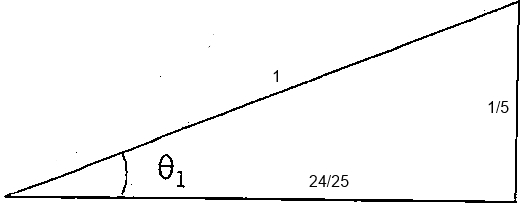
\includegraphics[width=0.4\textwidth]{figs/ckmfig1.jpg}
\caption{Cabibbo angle $\theta_c$. Lengths represent decay amplitudes}
\label{cabibbo}
\end{figure}


Only one thousandth of the $4\%$ deviation here is accountable from the 3rd generation but for the moment lets look a bit more into the first two.
When we get to it these subtle effects arising from the 3rd generation is where are theory upon CP violation developed from. From figure [a] we note that the transition within a generation $u\rightarrow d$ is calculated as $\cos\theta$ and across the generation as $\sin\theta$ which actually corresponds to $u\rightarrow s$. If we were naive enough to presume only two generations of matter existed we would construct an amplitude matrix of the corresponding transitions based on this, as we will demonstrate now. Note that, for the moment, anti-particles have amplitudes that are the same as their matter counterparts.[4]

\[  \left( \begin{array}{ccc} 
A_{ud} & A_{us} \\
A_{cd} & A_{cs}  \\
\end{array} \right)
 = \left( \begin{array}{ccc}
 cos\theta_{c} & sin\theta_{c} \\
 -sin\theta_{c} & cos\theta_{c} \end{array} \right) \]

From our diagram we see that the $\theta_c\sim 12^{\circ}$ experimentally this is measured $\theta_c = 13.1^{\circ}$ [?].The impact of this was that the decay rate of many hadronic particles could be calculated akin to lepton decays with the additional factor of $cos\theta_c$or $sin\theta_c$ in the matrix element. At a quick glance of the Weak Lagrangian [insert fancy lagrangian WL] we see the interaction term is a key element in the vertexes of our Feynman diagram describing the interactions. An element of this the $\gamma$ signifies axial vector coupling with properties which contribute to CPV [ref].

\begin{figure}[h]
\centering
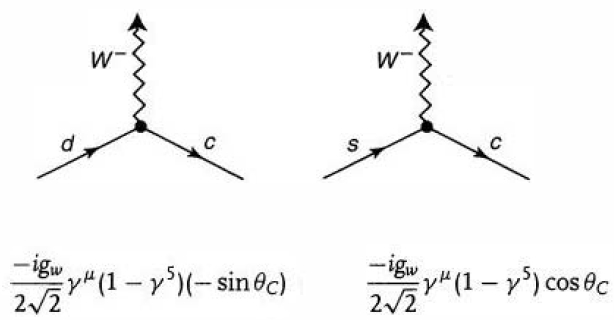
\includegraphics[width=0.5\textwidth]{figs/ckmfig2.jpg}
\caption{Decay amplitudes across generations. Left $d\rightarrow c$ and right $s\rightarrow c$.}
\label{fey1}
\end{figure}


To progress onto a mechanism for mixing 3 generations of quarks we must look further into what sets the Weak interacting quarks apart from the quarks we associate with electromagnetic and strong interactions. To begin let us look at an example of the kaon decay into two muons.
 
\begin{figure}[h]
\centering
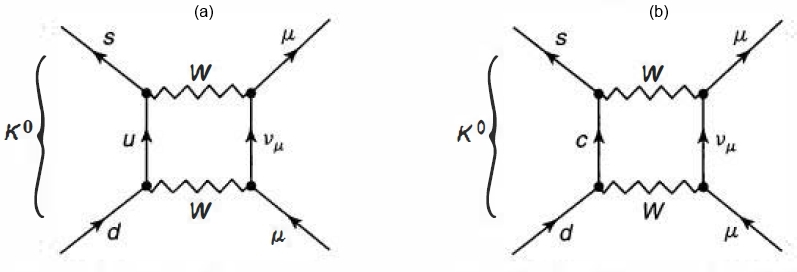
\includegraphics[width=0.5\textwidth]{figs/ckmfig3.jpg}
\caption{Kaon Interfering Feynamn diagrams illustrating GIM mechanism (left - a, Right -b)}
\label{fey2}
\end{figure}


So for a decay scheme as the Kaon in [3.a] , we find a virtual up quark transmitted between the down and s. This is what would be know as a second order diagram as the direct decay to a W boson is forbidden.
When the amplitdes are found the branching ratio between that and the $K^+\rightarrow\mu\nu$ is calculated to be,
 \[\frac{K^0\rightarrow\mu\mu}{K^+\rightarrow\mu\nu}=10^{-8}.\]
However experimentally this value is found to be too high. What could also be possible is the diagram in [3.b] where our virtual quark is now charm. When we account for these two process we find that in [3.a] the amplitude is proportional to $sin\theta_c cos\theta_c$ and in [3.b] the amplitude is proportional to $-sin\theta_c cos\theta_c$ on account of $A_{cd}$ in our simple matrix above. 
In 1970, what is called the (Glashow, Iliopoulos and Maiani) GIM mechanism was responsible for a solution, it proposed that throuh the interference with another order diagram there would be a near cancellation. The remaining value come from the difference in mass between the up and charmed quark. Using the experimental Amplitudes this allowed calculation provide a clear prediction for the mass of the charmed quark of about $1.5GeV$ which was discovered in 1974.
 
Cabibbo's theory of mixing together with the GIM mechanism allows us to look at quarks from a different perspective. Instead of one quark that feels the strong, electromagnetic and weak force, we have a sort of mixed phase of quarks involve in weak interactions. So a weak d and s are given by,

\[d' =dcos\theta_c +scsin\theta_c\] and
\[s'=scos\theta_c -sin\theta_c.\]

We can then formulate these in a matrix,

%\[ \left( \begin{array}{c} d' \\  s' \end{array} \right)  = \left( \begin{array}{ccc} cos\theta_c & sin\theta_c \\ -sin\theta_c & %cos\theta_c \end{array}\right) \left( \begin{array}{c} d \\  s \end{array} \right) \]

Now it the following doublets are found [assumed?] like in leptons using an analogous cabibbo rotated states

\[\left( \begin{array}{c}
 u \\ d'
 \end{array} \right)  = 
\left( \begin{array}{c}
 u \\ dcos\theta_c +ssin\theta_c
 \end{array} \right) \mbox{ and }
 \left( \begin{array}{c}
 c \\ s' \\
 \end{array} \right)  =
 \left( \begin{array}
{c} c \\
 s\cos\theta_c -d \sin\theta_c \\
 \end{array}
\right)
\]

Moving onto a third generation of quarks we repeat the method of finding mixing angles from the Amplitude triangles.

\begin{figure}[h]
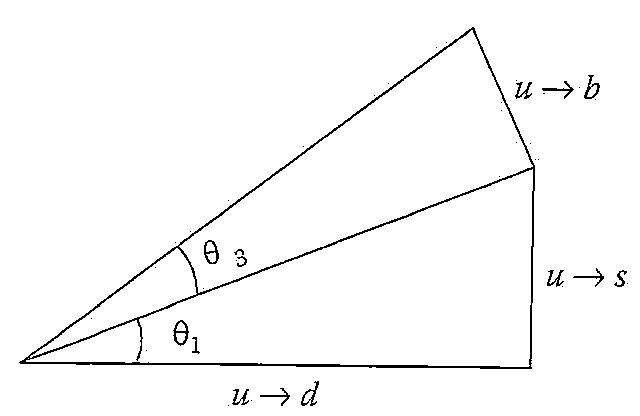
\includegraphics[width=0.3\textwidth]{figs/ckmfig4a.jpg}
\caption{Mixing triangle across 3 generations}
\label{tri3}
\end{figure}
\begin{figure}[h]
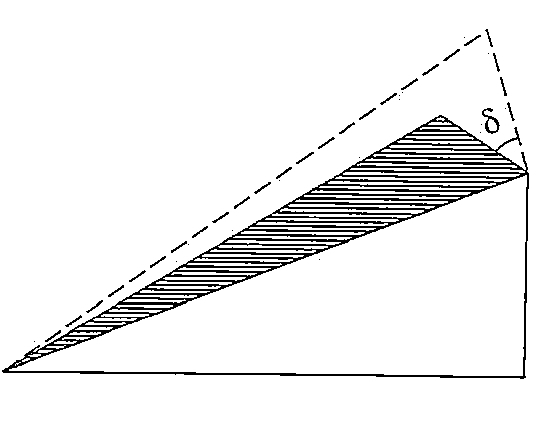
\includegraphics[width=0.3\textwidth]{figs/ckmfig4b.jpg}
\caption{Complex phase in the 2nd to 3rd generation transitions}
\label{tri4}
\end{figure}

In \cref{tri3} we have now an additional triangle with its base atop the hypotenuse of the 1st to 2nd generation triangle. The transition now facilitates the Amplitude of the up quark transitioning along the bottom quark path. This gives rise to the angle $\theta_3$ a mixing angle between the 1st and 2nd generation on this logic the mixing angle between the 2nd and 3rd is $\theta_2$. Our pictorial representation has another hidden feature of it. The plane the triangle sits in can be thought of as the ‘matter-antimatter mirror’ and our upper right-angle triangle can swing in and out of the page at an angle. It is called the Kobayashi-Maskawa phase, where $\delta=0$ is on the plane of the triangle below. This parameter can set a difference between quarks and antiquarks which we will later see and may be the clue to the source of CP violation in nature, but that remains to be seen since  conditions are in place to allow for CP violation , $\delta\neq0$,$\pi$ or $\theta_i\neq0,\frac{\pi}{2}$ .  [7].
With a full catalog of mixing between quarks we can scale our prior models to a 3x3 matrix incorporating every type of quark mixing in the original formalism [6]. 

\[V_{CKM} = \left( \begin{array}{ccc} V_{ud} & V_{us} & V_{ub} \\ V_{cd} & V_{cs} & V_{cb} \\ V_{td} & V_{ts} & V_{tb} \end{array}\right) = \left( \begin{array}{ccc} c_1 & s_1 c_3 & s_1 s_3 \\ -s_1 c_2 & c_1 c_2 c_3 -s_2 s_3 e^{i\delta} & c_1 c_2 s_3 + s_2 c_3 e^{i\delta} \\ -s_1 s_2 & c_1 s_2 c_3 +c_2 s_3 e^{i\delta} & c_1 s_2 s_3 - c_2 c_3 e^{i\delta} \end{array} \right). \]

In order to take advantage of the CKM matrix to illuminate CP violating decays we must have two weak amplitudes with complex phase components. A quick example of such would be the a 4 quark system [7]. Consider two up quarks i and k and two down quarks j and l. We find that the matrix element is,

\[M=(V_{ij} V_{kl}) A_1 e^{i \delta_{1}} +(V_{il} V_{kj}) A_2 e^{i\delta_{2}}\] 

Where $A_1$ and $A_2$ are real value amplitudes where each one represent a unique initial state transitioning to the same final states .The $\delta_1$ and $\delta_2$ are the phases due to higher order processes. The difference between them may be defined as the $\Delta\delta = \delta_1 - \delta_2$ and is known as the CP-even phase [ref]. If we perform the CP operation on this matrix element we obtain,
\[\overline{M}=(V_{ij} V_{kl})^* A_1 e^{i\delta_1} +(V_{il} V_{kj})^* A_2 e^{i\delta_2}\]

The two individual amplitudes $A_1$ and $A_2$ in each of the Matrix elements interfere with each other, so to simplify this down for a moment let us absorb the coefficients into $A_1$ and $A_2$ and solve for their decay rates. 
Let,

\[ \left|A\right|^2 = \left| A_1 +A_2 \right|^2\]
\[=\left|  A_1 \right|^2+ \left| A_2 \right|^2 +2\it{R} e\left| A^*_2 A_1 \right| \]
\[=\left| A_1 \right|^2 + \left| A_2 \right|^2 +2\left|A_1 A_2 \right| cos(\Delta \phi - \Delta\delta),\] and
\[\left| \overline{A}\right|^2 =\left| A_1 \right|^2+ \left| A_2 \right|^2 +2\left| A_1 A_2 \right| cos(\Delta \phi - \Delta\delta),\]

The $\phi$ in this case is the CP-even phase. We now define CP asymmetry as,

\[\mathbf{A}_{CP} = \frac{\left|A\right|^2-\left|\overline{A}\right|^2}{\left|A\right|^2-\left|\overline{A}\right|^2}\]

To find the Asymmetry in our four quark system we solve for the matrix elements. The result is,

\[ \mathbf{M}_{CP}= \frac{ 2\it{I}m (V_{ij} V_{kl} V^{*}_{kj }V^{*}_{il} )\sin(\Delta\delta) A_{1} A_{2}}{\left| V_{ij} V_{kl}\right|^2 A^{2}_{1} + \left|V_{kj}V_{il}\right|^2 A^{2}_{2} +2 \it{R} e (V_{ij} V_{kl} V^{*}_{kj} V^{*}_{il} ) \cos(\Delta\delta)A_1 A_2} \]

CP violation in this respect is proportional to $2\it{I}m(V_{ij}V_{kl}V^{*}_{kj}V^{*}_{il})$ which is called $\cal{J}$, the Jacobian. The Jacobian is just the gradient of the scalar valued CKM matrix it also is subject to the same CP violating conditions as what $\delta$ boasted.

So now we are stuck with the eternal burden of having a theory with an unknown number of free parameters to test with. To fix this we would like our CKM matrix to be unitary i.e. that itself by it's complex conjugate produces the Identity matrix. A quick glance and a brief frown reveals that the matrix thus far bare no hope unless our off-diagonal elements are relatively small. Hence since CP violation turns out to be very small experimentally and these off diagonal elements are in turn correlated to CPV we construct in close approximation a unitary matrix as such. We adopt the Wolfenstein parametrization [ref] where we expand on a small parameter $\lambda = 0.22$ to a power series,

\[ V_{W} =\left| \begin{array}{ccc} 1-\frac{\lambda^2}{2} & \lambda & A\lambda^3(\rho-i\nu) \\ -\lambda & 1-\frac{\lambda^2}{2} & A\lambda^2 \\ A\lambda^3(1-\rho-i\nu) &  -A\lambda^2 & 1 \end{array}\right| + \cal{O}(\lambda^4)\]

Looking back at the original $V_{CKM}$,

\[\lambda =s_{1} , A=\frac{s_{2}}{s^{2}_{1}}, \rho =\frac{s_{3}}{s_{1}s_{2}}\cos\delta \mbox{ and } \nu = \frac{s_3}{s_1}{s_2}\sin\delta.\]

Comparing this to experimentally measured values CKM matrix elements we have pretty close agreement.

\[V_{exp} = \left( \begin{array}{ccc} 0.9739-0.975 & 0.221-0.227 & 0.0029-0.0045 \\ 0.221-0.227 & 0.9730-0.9744 & 0.039-0.044 \\ 0.0048-0.01 &  0.037-0.043 & 0.9990-0.9992 \end{array}\right) + \cal{O}(\lambda^4)\]
[Can give an example of such a decay that provides direct CKM element values][8]

 As you can see there is a dependance on experimental data. An $n\times n$ complex matrix will have $n^2$ real and complex parameters while unitarity mean we have $n^2$ constrains. Since we have 6 quarks $(2n)$ which can all have independent phases we have $2n$ fewer parameters. Fixing one phase we then have $n^2 - (2n - 1)$. In the real unitary matrix we have n dimensions and $\frac{n(n-1)}{2}$ free parameters. Thus the total imanginary parameters in the CKM matrix is,
 \[n^2 - (2n - 1)-\frac{n(n-1)}{2} = \frac{(n-1)(n-2)}{2}\]
 which for n=3 is 1. Hence we have 4 unknown parameters in total, which is why we depend on experiments. [9]

As found in [9] 9 constraints are needed, 6 of which are the sum of complex terms which are zero by orthogonality. Here are three of these unitary relation equations, 
\[V_{ud}V^{*}_{us}+V_{cd}V^{*}_{cs}+V_{td}V^{*}_{ts}=0,\]
\[V_{us}V^{*}_{ub}+V_{cs}V^{*}_{cb}+V_{ts}V^{*}_{tb}=0,\]
\[V_{ud}V^{*}_{ub}+V_{cd}V^{*}_{cb}+V_{td}V^{*}_{tb}=0,\]

We visualize these as Unitary triangles in the complex plane and have an surface area of $\frac{\left|\cal{J}\right|}{2}$. The area is then non-zero for CP violating weak interactions.

\begin{figure}[h]
\centering
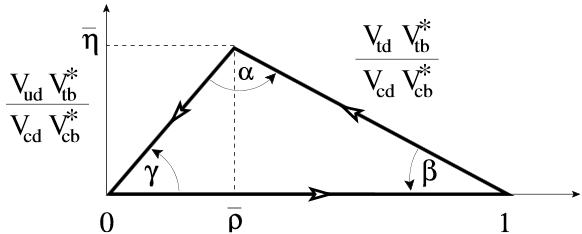
\includegraphics[width=0.5\textwidth]{figs/ckmfig5.jpg}
\caption{Unitary Triangle with angles $\alpha, \beta \mbox{ and } \gamma$}
\label{tri4}
\end{figure}

We now look a bit more closely at the 3rd unitary equation and construct the appropriate triangle. In figure {5}[10] we form a triangle on the basis (x,y) with corners at (0,0), (1,0) and ($\overline{\rho},\overline{\nu}$) where the reparametrizations are,

\[\overline{\rho}=\rho\left(1-\frac{\lambda^2}{2}\right) \mbox{ and } \overline{\nu}=\nu\left(1-\frac{\lambda^2}{2}\right)\]
The three angles in this diagram $\alpha , \beta and \gamma$ are defined as,

\[ \alpha\equiv arg\left(-\frac{V_{tb}V^{*}_{tb}}{V_{ud}V^{*}_{ub}}\right) =\frac{1}{2}\sin^{-1}\left(\frac{2\overline{\nu}(\overline{\nu}^2+\overline{\rho}^2-\overline{\rho})}{(\overline{\rho}^2+\overline{\nu}^2)((1-\overline{\nu})^2+\overline{\nu}^2)}\right) \]

\[\beta\equiv argl\left(-\frac{V_{cd}V^{*}_{cb}}{V_{td}V^{*}_{tb}}\right) = \frac{1}{2}\sin^{-1}\left(\frac{2\overline{\nu}(1-\overline{\rho})}{(1-\overline{\rho})^2+\overline{\rho}^2}\right)\]

\[\gamma\equiv arg\left(-\frac{V_{ud}V^{*}_{ub}}{V_{cd}V^{*}_{cb}}\right) = \frac{1}{2}\sin^{-1}\left(\frac{2\overline{\rho}\overline{\nu}}{\overline{\rho}^2+\overline{\nu}^2}\right)\]
,and $\alpha + \beta + \gamma = 180^{\circ}$. Direct measurement of these angles is performed by observations of CP violations in B meson decays which shall be covered in the following section.


%\end{document}
